\newcommand{\sxx}{\sum_{i=1}^n x_i^2 - n\overline{x}^2}
\newcommand{\sxy}{\sum_{i=1}^n x_i Y_i - n\overline{x}\overline{Y}}
\newcommand{\syy}{\sum_{i=1}^n Y_i^2 - n\overline{Y}^2}
\newcommand{\ssr}{\sum_{n=1}^n (Y_i - A - Bx_i)^2}

\chapter{Regressione Lineare}

\section{Teoria}

\subsection{Test Non Parametrici}

{\color{gray} Questa sezione è trattata in questo capitolo nonostante a livello teorico appartenesse al precedente perché sulla regressione ci sono pochi esercizi e quindi l'esercitatrice ha unito i due argomenti} \n

\ind Nei test parametrici non si fanno inferenze sui parametri ma sulla distribuzione di una o più popolazioni. Un esempio è il test Chi-quadro di buon adattamento, dove vogliamo sapere se la popolazione ha una certa distribuzione assegnata. \n

\ind \textbf{Test $\chi^2$ di buon adattamento}: prendiamo un insieme di dati che vogliamo analizzare e supponiamo una certa distribuzione che ci aspettata se i dati fossero distribuiti in modo casuale. Il test confronta la distribuzione effettiva dei dati con quella attesa e ci dice se ci sono differenze significative tra le due. In conclusione, se i dati che abbiamo raccolto sono simili a quelli che ci aspetteremmo in base alla nostra ipotesi, allora il test ci darà un valore basso, altrimenti ci darà un valore alto. \n

\ind \textbf{Osservazione}: Il test chi-quadro può essere effettuato in 3 contesti diversi:
\begin{enumerate}
    \item Caso in cui la popolazione ha distribuzione discreta finita
    \item Caso in cui la popolazione ha distribuzione discreta infinita
    \item Caso in cui la popolazione ha distribuzione continua
    \item Confronto con una distribuzione assegnata a meno di parametri incogniti
\end{enumerate}

\ind \textbf{Osservazione}: Per poter applicare il test nei casi continui o con dati infiniti, sarà fondamentale raggruppare i dati. \n

\ind \textbf{Definizione}: Per poter applicare la procedura del test per una distribuzione discreta, affinché ci sia buona approssimazione devono essere soddisfatte le due condizioni della \textit{regola empirica}:
\begin{enumerate}
    \item $f_k > 1 \quad \forall k = 1, ..., j$
    \item $f_k \geq 5$ per l'80\% dei K
\end{enumerate}

\ind \textbf{Osservazione}: Se i dati non verificano la regole empirica andrebbero raggruppate le classi. \n

\subsection{Richiami di Statistica Descrittiva - Dati accoppiati}

Abbiamo un campione in cui osserviamo due variabili accoppiate $(x_1, Y_1), ..., (x_n, y_n)$. Abbiamo 2 metodi per misurare il legame: 
\begin{itemize}
    \item graficamente: diagramma di dispersione
    \item numericamente: coefficiente di correlazione lineare: $$ r_{x,y} = \dfrac{1}{n-1} \dfrac{\sum_{i=1}^n (x_i - \overline{x}(y_i - \overline{y}}{s_x s_y}$$
\end{itemize}

\ind \textbf{Osservazione}: Il coefficiente di correlazione lineare assume valori r$\in [-1, 1]$. Nello specifico diremo che:
\begin{itemize}
    \item $|r_{x,y}|$ vicino a 1: avremo forte legame tra x e y
    \item $|r_{x,y}|$ vicino a 0: avremo poco legame tra x e y.
\end{itemize} 

\ind \textbf{Obiettivo}: L'idea ora è di trovare la retta di equazione $y= a + bx$ che\textit{meglio approssima} i dati nel diagramma di dispersione, ovvero che minimizza le distanze al quadrato tra $y_i$ valore osservato e $a + bx_i$ valore previsto fissata la retta. \n

\ind \textbf{Definizioni}: $(y_i - a - bx_i)^2$ è lo \textit{scarto quadratico} tra il valore osservato $y_i$ e il valore previsto $a + bx_i$. Lo \textit{scarto quadratico totale} è la sua sommatoria: $$\sum_{i=1}^n (y_i - a - bx_i)^2$$ 

\ind \textbf{Osservazione}: Per trovare a e b in modo da minimizzare lo scarto quadratico totale. Troveremo:
\begin{itemize}
    \item $b = \dfrac{r_{x,y}}{s_x} s_y$
    \item $a = \overline{y} - b\overline{x}$
\end{itemize}

\ind \textbf{Definizione}: Con questi valori di a e b la retta prende il nome di \textit{retta di regressione di y su x}

\subsection{Modello di Regressione Lineare Semplice}

\textbf{Obiettivo}: Finora abbiamo confrontato 2 variabili, ora si tratta di studiare la \textit{dipendenza} tra esse.  \n 

\ind \textbf{Definizione}: Vogliamo studiare la \textit{distribuzione di y} per ogni fissato valore della variabile x:
\begin{itemize}
    \item x è detta \textit{ingresso} o predittore o input
    \item y è detta \textit{uscita} o risposta o output
\end{itemize}

\ind \textbf{Osservazione}: Si assume che il legame tra input ed output sia lineare a meno di un errore: $$Y_i = \alpha + \beta x_i + e_i \qquad e1, ..., e_n \text{ i.i.d}$$ Dunque avremo $x_i, \alpha, \beta$ fissati, mentre $e_i$ essendo l'errore è una variabile aleatoria, e di conseguenza $Y_i$ è una variabile aleatoria. \n

\ind \textbf{Definizione}: Si assume che $e_i \sim N(0, \sigma^2)$ e quindi $$Y_i \sim N(\alpha + \beta x_i, \sigma^2)$$ con $\alpha, \beta, \sigma^2$ parametri incogniti. L'obiettivo è di fare inferenze sui parametri incogniti. \n 

\ind \textbf{Definizione}: Supponiamo di non aver fatto ancora osservazioni, vogliamo trovare degli stimatori di $\alpha, \beta$. Usiamo A e B, detti \textit{stimatori dei minimi quadrati di $\alpha$ e $\beta$}. Denotiamo con:
\begin{itemize}
    \item $S_{xx}$ somma dei quadrati di x: $\sxx$
    \item $S_{YY}$ somma dei quadrati di Y: $\syy$
    \item $S_{xY}$ somma dei prodotti incrociati tra x e Y: $\sxy$
\end{itemize} 
Allora definiamo: $$B = \dfrac{S_{x,Y}}{S_{xx}} \qquad A= \overline{Y} - B\overline{x}$$

\ind \textbf{Definizione}: Siamo riusciti a dare una stima puntuale, per poter dare la stima intervallare e il test di ipotesi serve conoscere la \textit{legge di A e B}:$$B = \dfrac{1}{S_{xx}} \left( \sum_{i=1}^n x_iy_i - n \overline{x}\overline{Y} \right) \sim N \left(\beta, \dfrac{\sigma^2}{S_{xx}} \right)$$ $$A = \overline{Y} - B\overline{x} \sim N \left( \alpha, \dfrac{\sigma^2 \sum_{i=1}^n x_i^2}{n S_{xx}} \right)$$

\ind \textbf{Definizione}: Queste due formule ci permettono di trovare la \textit{stima per $\sigma^2$}. Consideriamo i \textit{residui}: $R_i = Y_i - A - Bx_i$, vogliamo trovare la loro legge. Prendo la formula di $Y_i : \alpha + \beta x_i + e_i$ , la standardizzo, la elevo al quadrato e trovo la Chi-quadro con n gradi di libertà. Se però uso due stime per $\alpha, \beta$ perdo due gradi di libertà. Definisco quindi la somma dei quadrati residui come $SS_R=\ssr$ e trovo la stima di $\sigma^2$: $$\dfrac{\ssr}{\sigma^2} \sim \chi^2(n-2)$$ Infine, dato che $E \left( \dfrac{SS_R}{\sigma^2} = n-2 \right)$ allora $ \left( \dfrac{SS_R}{n-1} = \sigma^2 \right)$. In conclusione, uno \textit{stimatore non distorto di $\sigma^2$} è $$\dfrac{SS_R}{n-2}$$

\subsection{Intervallo di Confidenza per $\beta$}

Dal fatto che $B \sim N(\beta, \frac{\sigma^2}{s_{xx}})$ segue che se tolgo beta e standardizzo ottengo una gaussiana: $$\dfrac{B - \beta}{\dfrac{\sigma}{\sqrt{S_{xx}}}} \sim N(0,1)$$ Essendo $\sigma^2$ incognito devo usare il suo stimatore $\dfrac{SS_R}{n-2}$ . Allora ottengo: $$\sqrt{\dfrac{(n-2)S_{xx}}{SS_R}} (B - \beta) \sim t(n-2)$$ Siamo riusciti ad ottenere una statistica con legge che non dipende dai parametri incogniti. \n

\ind \textbf{Definizione}: Troviamo l'intervallo di confidenza di $\beta$ di livello $(100 - \gamma)$: $$IC = \left( \hat{\beta} - \sqrt{\dfrac{SS_R}{S_{xx}(n-2)}}t_{n-2},\sfrac{\gamma}{2}, \hat{\beta} + \sqrt{\dfrac{SS_R}{S_{xx}(n-2)}}t_{n-2},\sfrac{\gamma}{2} \right) $$

\ind \textbf{Osservazione}: La semiampiezza dell'IC per $\beta$ dipende dai dati campionari perché è data dalla somma dei quadrati residui $SS_R$ che a sua volta dipende da $y_1, ..., y_n$ \n

\subsection{Verifica dell'ipotesi $\beta=0$}

L'ipotesi nulla $H_0: \beta = 0$ equivale a dire che l'output \textit{non dipende} dall'input. Se i dati sperimentali conducono al rifiuto di $H_0$ è possibile concludere che la dipendenza tra input ed output sia significativa. \n

\ind \textbf{Definizione}: Se vale $H_0$ e quindi $\beta=0$ allora ottengo $$\sqrt{\dfrac{(n-2)S_{xx}}{SS_R}} (B - 0) \sim t(n-2)$$ Dunque la mia \textit{regione critica} sarà: $$ \abs{\sqrt{\dfrac{(n-2)S_{xx}}{SS_R}}\hat{\beta}} > t_{n-2, \sfrac{\gamma}{2}}$$

\subsection{Regressione verso la Media}

Esiste un fenomeno di regressione verso la media, dove si nota che i caratteri più "estremi", passando di padre in figlio diventano meno "estremi". \n

\ind \textbf{Definizione}: Per concludere con un test statistico che i dati denotano regressione verso la media, si sceglie come ipotesi alternativa $H_1: \beta < 1$, in modo tale che se i dati permettono di rifiutare l'ipotesi nulla, ovvero accettiamo $H_1$, allora troviamo \textit{regressione verso la media}. Dato che l'ipotesi nulla $H_0: \beta \geq 1$ ma sappiamo che $0 \leq \beta \leq 1$ allora la nostra ipotesi nulla sarà $H_0 : \beta = 1$, permettendoci di calcolare la sua regione critica come:  $$ \sqrt{\dfrac{(n-2)S_{xx}}{SS_R}}(\hat{\beta}-1) < - t_{n-2, \gamma}$$

\subsection{Coefficiente di Determinazione}

\textbf{Obiettivo}: misurare la variazione degli output corrispondenti agli input. \n

\ind \textbf{Osservazione} Le $Y_i$ variano perché gli input non sono tutti uguali e per il fatto che abbiamo nella formula di $Y_i$ un errore $e_i \sim N(0, \sigma^2)$ \n

\ind \textbf{Definizione}: Si ha che $S_{YY} - SS_R$ è la variazione dell'output quantificata dai valore dell'input, in quanto $SS_R$ è la quantità residua di variazione della risposta. Allora troviamo il \textit{coefficiente di determinazione} come $$R^2 = 1 - \dfrac{SS_R}{S_{YY}}$$ definita come la proporzione della variazione dell'output che è qualificata dagli input: $0 \leq R^2 \leq 1$.
\begin{itemize}
    \item $R^2$ vicino a 1: maggior parte della variazione delle risposte giustificata dai produttori
    \item $R^2$ vicino a 0: solo una piccola parte della variazione delle risposte è giustificata dai produttori
\end{itemize}
\newpage
\section{Pratica}

\subsection{Esercizi}

\subsubsection{Test chi-quadro di adattamento - Discreta Finita}

\textbf{Traccia}: Un campione casuale di 100 assenza di studenti sono ripartiti tra i giorni della settimana come segue: Lunedì=27, Martedì=19 Mercoledì=13 Giovedì=15 Venerdì=26. Verifica l'ipotesi che un'assenza abbia la stessa probabilità di capire in un qualunque dei 5 giorni. \n

\ind \textbf{Soluzione}: 
\begin{enumerate}
    \item \textit{Distinzione discreta/continua}: Siamo nel caso di una distribuzione discreta: $$ \pi = (\pi_1, \pi_2, \pi_3, \pi_4, \pi_5) = (\sfrac{1}{5}, \sfrac{1}{5}, \sfrac{1}{5}, \sfrac{1}{5}, \sfrac{1}{5}) $$
    \item \textit{Calcolo frequenze assolute attese}: $$f_i = n \pi(i) = 100 \frac{1}{5} = 20$$ 
    \item \textit{Controllo Regola empirica}: RE soddisfatta: $f_k > 1 \quad \forall k = 1, ..., j
    \quad f_k \geq 5$ 80\% dei K
    \item \textit{Formulo ipotesi nulla ed alternativa}: Le nostre ipotesi sono: $$H_0: \text{la popolazione ha distribuzione } \pi$$ $$H_1: \text{la popolazione non ha distribuzione }\pi$$
    \item \textit{Trovo statistica e regione critica}: Guardo dal formulario, la statistica è sempre quella, la regione critica cambia se abbiamo parametri incogniti. In questo caso avremo: $$\text{Statistica: } Q = \sum_{j=1}^5 \dfrac{(N_j - f_j)^2}{f_j} \sim \chi^2(4)$$ $$\text{Regione Critica: } q=\sum_{j=1}^5 \dfrac{(n_j - f_j)^2}{f_j} \sim \chi^2_{4, \alpha}  $$
    \item \textit{Calcolo e Concludo}: Scelgo $\alpha=5\%$, trovo la regione critica: $$q = \dfrac{(27 - 20)^2}{20} + ... + \dfrac{(26 - 20)^2}{20} = 8$$ Trovo nelle tabelle $\chi^2_{4, 0.05}=9.49$ e quindi dato che $8 \ngtr 9.49$ accetto $H_0$, ovvero la popolazione ha distribuzione $pi$ a livello 5\%. I dati non sono in contraddizione significativa con $H_0$
    
\end{enumerate}

\subsubsection{Test chi-quadro di adattamento - Discreta Infinita}

\textbf{Traccia}: Da un'indagine eseguita qualche anno fa si sa che il numero di difetti di un macchinario prodotto dalla fabbrica PSI segue una distribuzione di Poisson di parametro $\lambda=1.76$. Vengono esaminati oggi 50 macchinari della fabbrica PSI ottenendo i dati relativi ai difetti: 10 senza, 14 ne mostrano uno, 15 ne mostrano due, 5 ne mostrano tre, 3 ne mostrano quattro e 3 ne mostrano 5 o più.

\textbf{Soluzione}
\begin{enumerate}
    \item \textit{Distinzione discreta/continua}: Abbiamo una v.a. discreta, nella precisione una Poisson.
    \item \textit{Calcolo le $\pi$}: Utilizziamo la formula della densità discreta della Poisson e troviamo: 
    \begin{itemize}
        \item $\pi_0 = e^{-176} \sim 0.172$
        \item $\pi_1 = e^{-176} 1.76 \sim 0.172$
        \item $\pi_2 = e^{-176} \sfrac{(1.76)^2}{2!} \sim 0.172$
        \item $\pi_3 = e^{-176} \sfrac{(1.76)^3}{3!} \sim 0.172$
        \item $\pi_4 = e^{-176} \sfrac{(1.76)^4}{4!} \sim 0.172$
        \item $\pi_5 = 1 - P(Y < 5) = 0.034$
    \end{itemize}
    \item \textit{Calcolo frequenze assolute attese}: Ottengo le frequenze assolute moltiplicando i precedenti valori per il numero di osservazioni, ovvero 50:
    \begin{itemize}
        \item $f_0= 8.6$
        \item $f_1= 15.15$
        \item $f_2= 13.3$
        \item $f_3= 7.8$
        \item $f_4= 3.45$
        \item $f_5= 1.7$
    \end{itemize}
    \item \textit{Controllo regola empirica}: I casi 4 e 5 non soddisfano il secondo punto della regola empirica, dunque li raggruppiamo ed otteniamo i nuovi valori: $\pi_4 \sim 0.103$ e $f_4 = 5.15$
    \item \textit{Formulo ipotesi nulla ed alternativa}: Le nostre ipotesi sono: $$H_0: \text{la popolazione ha distribuzione } \pi$$ $$H_1: \text{la popolazione non ha distribuzione }\pi$$
    \item \textit{Statistica e Regione Critica}: Calcolo la regione critica $q=\dsum_{j=1}^4 \dfrac{(n_j - f_j)^2}{f_j}$ e trovo 1.677, calcolo il chi-quadro $\chi^2_{4, 0.05}$ e trovo 9.49.
    \item \textit{Calcolo e concludo}: Accetto $H_0$ in quanto i dati sperimentali non sono in contraddizione significativa.
\end{enumerate}

\subsubsection{Test chi-quadro di adattamento - Continua e Stima Parametro}

\textbf{Traccia}: Una ditta di martinetti idraulici vuole analizzare la durata del modello PSI in commercio da 5 anni. Si analizza un campione di 10 pezzi ottenendo i tempi intercorsi dalla consegna al guasto:
\begin{center}
    \item $[0,299] = 55 $
    \item $[300, 599] = 25 $
    \item $[600, 899] = 10$ 
    \item $[900, 1199] = 4$
    \item $[1200, 1499] = 3$ 
    \item $[1500, 1799] = 2$ 
    \item $[1800, 1825] = 1$ 
\end{center}
Si può affermare che il tempo di vita segue una legge esponenziale?

\ind \textbf{Soluzione}
\begin{enumerate}
    \item \textit{Distinzione discreta/continua}: Siamo nel caso continua, avendo una $exp(\lambda)$. Non sappiamo il valore di $\lambda$, ma essendo $E[X] = \sfrac{1}{\lambda}$ lo stimiamo con $\sfrac{1}{\overline{x}_100}$
    \item \textit{Calcolo $\lambda$}: Per calcolare il valore medio devo prendere il punto medio delle classi e le rispettive frequenze. Ottengo $$\overline{x}_100 = \frac{1}{100}(55 \cdot 150 + ... + 1 \cdot 1813) = 403.63 $$ Allora la mia stima di $\lambda$ è 0.002477. 
    \item \textit{Calcolo frequenze assolute attese}: 
    \begin{itemize}
        \item $[0,299] = P( Y < 300) = 1 - e^{-0.002477 \cdot 300} = 0.524 $
        \item $[300, 599] = P(300 \leq Y < 600) = 0.249 $
        \item $[600, 899] = 0.119$ 
        \item $[900, 1199] = 0.056$
        \item $[1200, 1499] = 0.027$ 
        \item $[1500, 1799] = 0.013$ 
        \item $[1800, 1825] = 0.001$ 
    \end{itemize}
    \item \textit{Controllo regola empirica}: La regola empirica non è soddisfatta, allora raggruppo gli ultimi 3 casi ottenendo $0.052$
    \item \textit{Calcoli e Concludo}: Gli altri punti sono uguali ai precedenti esercizi, con l'unica osservazione che in questo esercizio avrò una $\chi^2(5-1-1)$ in quanto ho stimato il parametro $\lambda$ e quindi perdo un grado di libertà. Avrò $2.6 > 7.981$ dunque ai dati non sono in contraddizione significativa con $H_0$
\end{enumerate}

\subsubsection{Regressione Lineare}

\textbf{Traccia}: Si consideri il seguente campione di n=9 osservazioni relative ai caratteri X e Y:
\begin{center}
    \item X  17 8 36 23 19 17 2 5
    \item Y 25 0 11 -26 -2 -18 8 26 35
\end{center}
Supponendo valga un modello di regressione lineare semplice $$Y = \alpha + \beta x + e$$
\begin{enumerate}
    \item Tracciare il grafico di dispersione dei dati, calcolare il coefficiente di correlazione lineare e la retta di regressione di Y su X.
    \item Costruire un IC al livello 99\% per $\beta$
    \item Verificare l'ipotesi $\beta=0$ a livello 1\% 
    \item Calcolare una misura della bontà di adattamento del modello
    \item Discutere il grafico dei residui della regressione di Y su X
\end{enumerate}

\ind \textbf{Soluzione punto 1} 
\begin{itemize}
    \item Il grafico di dispersione sarà: 
        \begin{figure}[H]
            \centering
            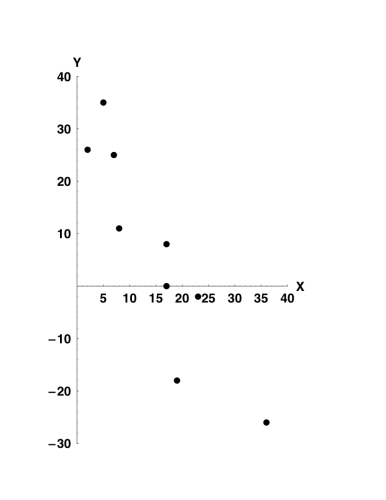
\includegraphics[scale=.5]{Foto/cr.png}
        \end{figure}
    \item La formula per calcolare il coefficiente di correlazione lineare è $$r_{xy}= \dfrac{s_{xy}}{\sqrt{s_{xx}s_{yy}}}$$. Calcolo allora $\overline{x}_9= 14.89$ e $\overline{y}_9= 6.56 $ e trovo $$r = \dfrac{-1576.44}{\sqrt{910.89 \cdot 3328.22}} = - 0.9$$ Troviamo quindi una forte correlazione lineare negativa.
    \item Trovo la retta di regressione di Y su X con la formula $y = \hat{\beta}x + \hat{\alpha}$. Trovo $\beta = \frac{S_{xy}}{S_{xx}} = \frac{-1576.44}{910.89} = -1.73$ e $\alpha = \overline{y} - \hat{\beta}\overline{x} = 6.56 - (-1.73) \cdot 14.89 = 32.32$ e trovo quindi la retta $$y=  -1.73x + 32.32$$
\end{itemize}

\ind \textbf{Soluzione punto 2}: Dal formulario è $ \left( \hat{\beta} \pm \sqrt{\dfrac{SS_R}{S_{xx}(n-2)}} t_{n-2, \sfrac{\alpha}{2}} \right)$ Conosco n=9, $\alpha/2 = 0.005$, $\hat{\beta}= -1.73$, $S_{xx} = 910.89$, mi manca trovare, attraverso formulario e tabelle $SS_R=599.94$ e $t_{7, 0.005}=3.499$ Dunque l'intervallo è $$-1.73 \pm \sqrt{\dfrac{599,94}{7 \cdot 910.89}} = (-2.80, -0.66)$$

\ind \textbf{Soluzione punto 3}: $H_0 :\beta = 0 \quad H_1 : \beta \neq 0$. Rifiutiamo l'ipotesi nulla se (dal formulario) $$\abs{\sqrt{\dfrac{S_{xx} (n-2)}{SS_R} \hat{\beta}} > t_{n-2, \sfrac{\alpha}{2}}}$$ Calcolo e trovo che $5.64 > 3.499$ e quindi rifiuto $H_0$. Questo test si poteva fare anche osservando l'IC in quanto $$\beta \notin(-2.80, -0.66) $$

\ind \textbf{Soluzione punto 4}: Per calcolare la bontà di adattamento del modello si utilizza il coefficiente di determinazione: $$R^2 = 1 - \frac{SS_R}{S_{yy}}= 1 - \frac{599.94}{3328.22} = 0.82$$ Questo significa che l'82\% della variazione delle risposte è giustificata dai predittori, quindi dal modello. Osservazione: dal coefficiente di determinazione ritroviamo il quadrato del coefficiente lineare, che possiamo trovare in modulo. Per il segno, sappiamo che il coefficiente lineare ha lo stesso segno di $\beta$ \n

\ind \textbf{Soluzione punto 5}: Per calcolare i residui posso calcolarli con la formula $ \overline{e_i} = y_i - \alpha -\beta x_i $. Trovo allora
\begin{figure}
    \centering
    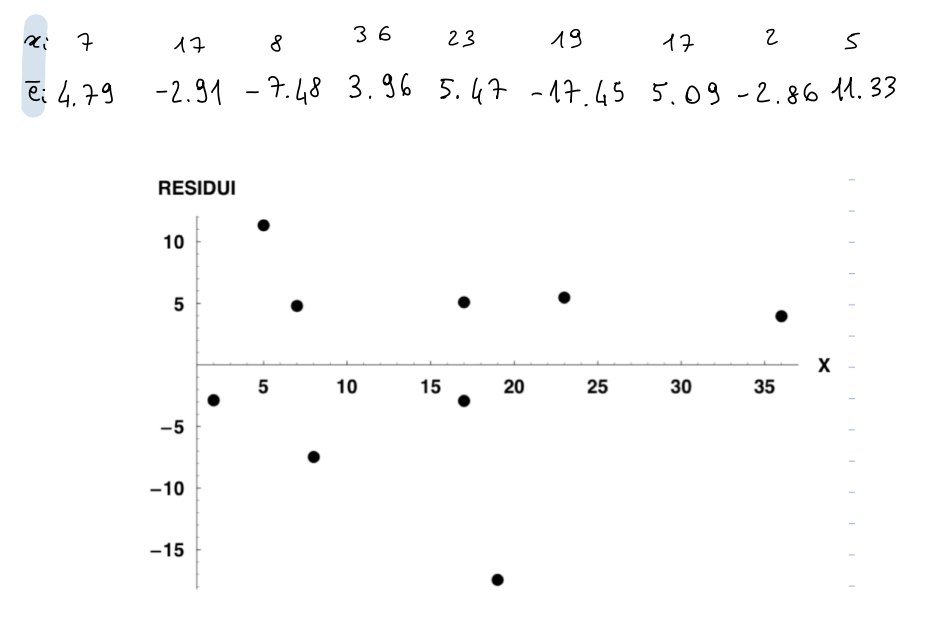
\includegraphics[scale=0.5]{Foto/c.png}
\end{figure}
I residui si dispongono in modo abbastanza casuale attorno all'asse x. 